% Chương 3
\chapter{PHƯƠNG PHÁP} % Tên của chương

\label{Chapter3} % Để trích dẫn chương này ở chỗ nào đó trong bài, hãy sử dụng lệnh \ref{Chapter1} 

%----------------------------------------------------------------------------------------

% Định nghĩa một số lệnh cần thiết để điều chỉnh định dạng cho một số nội dung nhất định trong bài
\renewcommand{\keyword}[1]{\textbf{#1}}
\renewcommand{\tabhead}[1]{\textbf{#1}}
\renewcommand{\code}[1]{\texttt{#1}}
\renewcommand{\file}[1]{\texttt{\bfseries#1}}
\renewcommand{\option}[1]{\texttt{\itshape#1}}

\section{Module 1 : Phát hiện dòng chữ trong văn bản}

\begin{figure}[H]
    \centering
    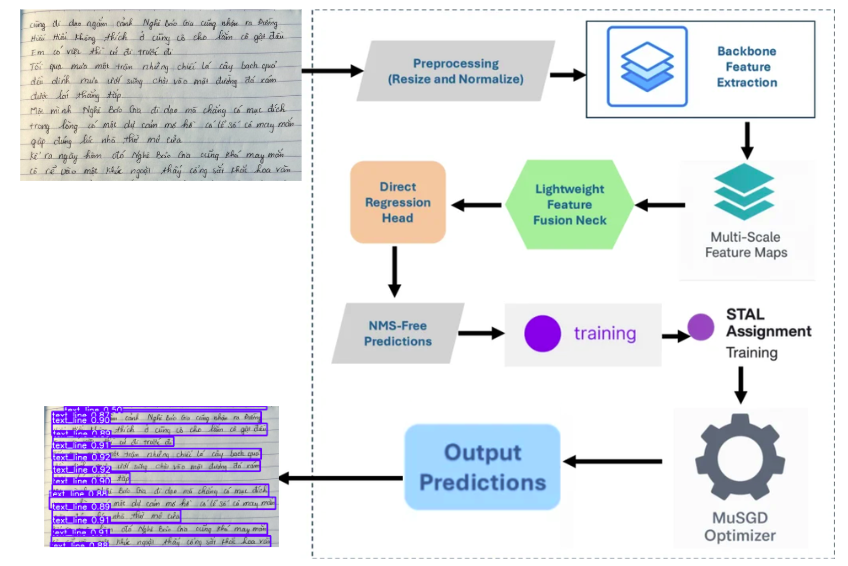
\includegraphics[width=0.9\linewidth]{Figures/Chapter3/Chapter3_3.png}
    \caption{Tổng quan quy trình phát hiện dòng chữ bằng YOLO26~\cite{Reference18}}
    \label{fig:handwriting_challenges}
\end{figure}

Quy trình xử lý của mô hình bắt đầu bằng việc tiền xử lý ảnh đầu vào thông qua các bước thay đổi kích thước (Resize) và chuẩn hóa điểm ảnh (Normalize) để tối ưu tính toán. Tiếp theo, dữ liệu được đưa qua mạng cơ sở (Backbone) nhằm trích xuất các bản đồ đặc trưng đa kích thước (Multi-Scale Feature Maps). Điều này giúp hệ thống linh hoạt nhận diện các dòng chữ có độ lớn và khoảng cách khác nhau. Các đặc trưng này sau đó được tổng hợp hiệu quả qua khối cổ hợp nhất tinh gọn (Lightweight Feature Fusion Neck) mà không làm tốn nhiều tài nguyên tính toán\cite{Reference19}.

Các đặc trưng sau khi dung hợp sẽ tiến thẳng vào đầu hồi quy (Direct Regression Head) để dự đoán trực tiếp tọa độ các dòng văn bản. Điểm đột phá của kiến trúc này là xuất ra kết quả mà không cần đến bước hậu xử lý phức tạp (NMS-Free Predictions), giúp triệt tiêu độ trễ và tăng tốc độ xử lý thực tế lên mức tối đa \cite{Reference18} Cuối cùng (Output Predictions), hệ thống trả về bức ảnh với các dòng chữ đã được khoanh vùng chính xác, đi kèm điểm độ tin cậy.

Riêng trong quá trình đào tạo (Training), mô hình sử dụng chiến lược gán nhãn thông minh (STAL) để đo lường sai số giữa dự đoán và thực tế. Dựa vào đó, thuật toán tối ưu hóa MuSGD sẽ tự động điều chỉnh các trọng số, giúp mạng lưới liên tục khắc phục lỗi và tăng cường độ chính xác sau mỗi chu kỳ học \cite{Reference18}.

\subsection{Chuẩn bị dữ liệu}
Tập dữ liệu gồm 660 ảnh văn bản tiếng Việt, được thu thập từ nhiều nguồn khác nhau nên mang tính đa dạng và gần với dữ liệu thực tế.

\begin{table}[h]
    \centering
    \begin{tabular}{lcc}
        \toprule
        \textbf{Tập dữ liệu} & \textbf{Số ảnh} & \textbf{Số nhãn} \\
        \midrule
        Train      & 506 & 506 \\
        Validation & 102 & 102 \\
        Test       & 52 & 52 \\
        \bottomrule
    \end{tabular}
    \caption{Thống kê tập dữ liệu.}
    \label{tab:dataset}
\end{table}

Trước hết, mỗi ảnh thường chứa nhiều dòng văn bản, với độ dài và khoảng cách giữa các dòng không đồng đều, gây khó khăn cho việc tách dòng và nhận diện. Bên cạnh đó, dữ liệu có sự khác biệt về góc chụp và bố cục, nhiều ảnh bị nghiêng hoặc lệch phối cảnh, làm tăng độ phức tạp trong xử lý.

Ngoài ra, kích thước và chất lượng ảnh không đồng nhất, bao gồm ảnh độ phân giải thấp, bị mờ hoặc nhiễu, ảnh hưởng đến quá trình trích xuất đặc trưng. Đặc biệt, dữ liệu tiếng Việt chứa nhiều dấu thanh và dấu phụ, các thành phần này nhỏ và dễ bị mất hoặc dính vào ký tự chính.

\subsection{Tiền xử lý dữ liệu}

\subsection*{1. Chiến thuật gán nhãn}
Thực hiện gán nhãn theo từng dòng chữ (line-level labeling), trong đó mỗi dòng văn bản được coi là một đơn vị độc lập.

Phương pháp thực hiện bao gồm việc sử dụng các công cụ gán nhãn chuyên dụng (Labeling Tools) để xác định và vẽ các hộp giới hạn (bounding boxes) bao quanh chính xác từng dòng chữ trong hình ảnh, đảm bảo dữ liệu đầu vào phù hợp cho quá trình huấn luyện mô hình.

\subsection*{2. Quy trình làm dữ liệu}

Quy trình được thiết kế theo dạng vòng lặp khép kín, kết hợp giữa tự động hóa và kiểm soát thủ công để tối ưu hóa hiệu suất:

\begin{figure}[H]
\centering

% Dùng resizebox để thu phóng tự động vừa khít chiều ngang trang giấy
\resizebox{\textwidth}{!}{
\begin{tikzpicture}[
    >={Stealth[length=2.5mm, width=1.5mm]}, % Kiểu mũi tên chuẩn
    base box/.style={
        rectangle, rounded corners=6pt,
        minimum width=3.4cm, minimum height=1.2cm,
        align=center, font=\sffamily\small\bfseries,
        line width=1pt
    },
    % Định nghĩa màu sắc cho từng loại block
    box input/.style={base box, fill=blue!5, draw=blue!60},
    box process/.style={base box, fill=cyan!5, draw=cyan!70},
    box bad/.style={base box, fill=red!5, draw=red!50},
    box trash/.style={base box, fill=gray!10, draw=gray!50},
    box hq/.style={base box, fill=green!5, draw=green!60},
    box lq/.style={base box, fill=orange!5, draw=orange!60},
    box manual/.style={base box, fill=purple!5, draw=purple!60},
    box train/.style={base box, fill=teal!5, draw=teal!70},
    box feedback/.style={base box, fill=magenta!5, draw=magenta!60},
    % Style đường kẻ bo góc mềm mại
    line/.style={->, draw=gray!60!black, line width=1.2pt, rounded corners=8pt}
]

% ===============================
% 1. ĐỊNH VỊ CÁC KHỐI (NODES)
% Khoảng cách ngang giữa các cột được giãn rộng để đường nối có không gian bẻ góc
% ===============================
\node[box input]   (text)   at (0, 0)      {Text Images};
\node[box process] (qf)     at (4.5, 0)    {Quality Filter};

\node[box bad]     (bad)    at (10, 2)     {Bad Images};
\node[box trash]   (rm)     at (15, 2)     {Remove};

\node[box process] (pad)    at (10, -2)    {PaddleOCR\\Detection};

\node[box hq]      (hq)     at (15, -0.5)  {High Quality};
\node[box lq]      (lq)     at (15, -3.5)  {Low Quality};

\node[box train]   (label)  at (20, -2)    {Label Dataset};
\node[box manual]  (man)    at (20, -5)    {Manual Fix};

\node[box train]   (train)  at (25, -2)    {Train YOLO26};
\node[box train]   (pred)   at (30, -2)    {Prediction};
\node[box train]   (err)    at (35, -2)    {Error Analysis};

\node[box feedback] (refine) at (30, -5)   {Refine Annotation};
\node[box feedback] (add)    at (30, 1.5)  {Add More Data};


% ===============================
% 2. VẼ CÁC ĐƯỜNG KẾT NỐI (EDGES)
% ===============================
% Luồng đầu vào
\draw[line] (text) -- (qf);

% Nhánh từ Quality Filter: ++(1.2,0) tạo một đoạn thẳng dài 1.2cm trước khi bẻ góc, giúp mũi tên không đâm vào khối
\draw[line] (qf.east) -- ++(1.2,0) |- (bad.west);
\draw[line] (qf.east) -- ++(1.2,0) |- (pad.west);

% Loại bỏ hình ảnh xấu
\draw[line] (bad) -- (rm);

% Phân nhánh từ PaddleOCR ra High/Low Quality
\draw[line] (pad.east) -- ++(0.8,0) |- (hq.west);
\draw[line] (pad.east) -- ++(0.8,0) |- (lq.west);

% OCR nhận diện quá tệ đẩy thẳng xuống Manual Fix
\draw[line] (pad.south) |- (man.west); 

% Nhánh High Quality đẩy thẳng vào Label Dataset (đã bỏ đường chéo nối xuống Manual Fix)
\draw[line] (hq.east) -- ++(1,0) |- (label.west);

% Nhánh Low Quality đẩy xuống Manual Fix
\draw[line] (lq.east) -- ++(1,0) |- (man.west);

% Từ Manual Fix hoàn thiện đẩy lên Label Dataset
\draw[line] (man.north) -- (label.south);

% Chuỗi Pipeline huấn luyện chính
\draw[line] (label) -- (train);
\draw[line] (train) -- (pred);
\draw[line] (pred) -- (err);


% ===============================
% 3. VÒNG LẶP PHẢN HỒI (FEEDBACK LOOPS)
% ===============================
% Vòng lặp 1: Error -> Refine Annotation -> Nối về Manual Fix
\draw[line, draw=magenta!80!black] (err.south) |- (refine.east);
\draw[line, draw=magenta!80!black] (refine.west) -- (man.east);

% Vòng lặp 2: Error -> Add More Data -> Nối về Train YOLO26
\draw[line, draw=magenta!80!black] (err.north) |- (add.east);
\draw[line, draw=magenta!80!black] (add.west) -| (train.north);

\end{tikzpicture}
}

\caption{Hình ảnh quy trình xử lý dữ liệu}
\label{fig:data_pipeline}

\end{figure}

\begin{enumerate}
    \item \textbf{Giai đoạn Sàng lọc}
    \begin{itemize}
        \item \textit{Text Images:} Tiếp nhận dữ liệu hình ảnh thô chứa văn bản.
        \item \textit{Quality Filter:} Phân loại chất lượng ảnh đầu vào. Những ảnh không đạt yêu cầu (\textit{Bad Images}) sẽ bị loại bỏ (\textit{Remove}).
    \end{itemize}

    \item \textbf{Giai đoạn Gán nhãn tự động}
    \begin{itemize}
        \item Sử dụng công cụ \textit{PaddleOCR Detection} để tự động nhận diện và tạo các nhãn bao quanh dòng chữ cho các ảnh đạt chất lượng \cite{Reference20}.
    \end{itemize}

    \item \textbf{Giai đoạn Kiểm định và Chỉnh sửa}
    \begin{itemize}
        \item \textit{High Quality:} Những ảnh được máy gán nhãn chính xác sẽ được chuyển thẳng vào tập dữ liệu nhãn (\textit{Label Dataset}).
        \item \textit{Low Quality / Manual Fix:} Những trường hợp máy nhận diện sai hoặc thiếu sẽ được chuyển qua bước chỉnh sửa thủ công bởi con người để đảm bảo độ chính xác tuyệt đối trước khi đưa vào tập dữ liệu.
    \end{itemize}

    \item \textbf{Giai đoạn Huấn luyện và Đánh giá}
    \begin{itemize}
        \item \textit{Train YOLO26:} Sử dụng tập dữ liệu đã gán nhãn chuẩn để huấn luyện mô hình YOLO26 \cite{Reference21}.
        \item \textit{Prediction:} Chạy mô hình trên dữ liệu thực tế để kiểm tra kết quả.
        \item \textit{Error Analysis:} Phân tích các lỗi sai của mô hình để thực hiện các bước cải tiến:
        \begin{itemize}
            \item \textit{Refine Annotation:} Tinh chỉnh lại các nhãn bị sai lệch.
            \item \textit{Add More Data:} Bổ sung thêm dữ liệu mới để tăng cường khả năng học của mô hình.
        \end{itemize}
    \end{itemize}
\end{enumerate}

\subsection{Hàm mất mát của YOLO26}

Hàm mất mát cốt lõi của YOLO26 được thiết kế lại hoàn toàn cho kiến trúc End-to-End (loại bỏ hậu xử lý NMS và module DFL) \cite{Reference18}. Tổng hàm mất mát $L_{total}$ là sự kết hợp có trọng số động giữa hàm phân loại ($L_{cls}$) và hàm hồi quy hộp bao ($L_{box}$):

\begin{equation}
L_{total}(t) = \lambda_{cls}(t) \cdot L_{cls} + \lambda_{box}(t) \cdot L_{box}
\end{equation}

Trong đó, $t$ là tiến trình huấn luyện (epoch hiện tại). Khác với các thế hệ trước, YOLO26 áp dụng cơ chế \textbf{ProgLoss (Progressive Loss Balancing)}: trọng số không cố định mà thay đổi theo thời gian. Ở giai đoạn đầu, mạng ưu tiên học phân loại đặc trưng ($\lambda_{cls}$ lớn), và về cuối quá trình, hệ thống tự động dồn trọng số để tinh chỉnh ranh giới tọa độ ($\lambda_{box}$ lớn)\cite{Reference19}.

\subsection*{1. Hàm phân loại với Nhãn mục tiêu mềm}

Để tối ưu hóa khả năng nhận diện các vật thể nhỏ (\textit{Small-Target-Aware}), YOLO26 không sử dụng nhãn cứng (đúng/sai tuyệt đối) mà dùng nhãn mềm $y_i$ để chấm điểm chất lượng thực tế của từng khung dự đoán:

\begin{equation}
L_{cls} = - \frac{1}{N} \sum_{i=1}^{N} \left[ y_i \cdot (1 - \hat{p}_i)^\gamma \log(\hat{p}_i) + (1 - y_i) \cdot \hat{p}_i^\gamma \log(1 - \hat{p}_i) \right]
\end{equation}

\begin{itemize}
    \item $N$: Tổng số lượng mẫu dữ liệu.
    \item $\hat{p}_i$: Xác suất dự đoán của mô hình.
    \item $y_i$: Điểm số mục tiêu mềm do cơ chế \textbf{STAL (Soft Target Assignment Loss)} gán tự động ($y_i \in [0, 1]$).
    \item $\gamma$: Hệ số hội tụ giúp giảm nhiễu từ các mẫu nền (mẫu âm tính dễ).
\end{itemize}

\subsection*{2. Hàm hồi quy hộp bao trực tiếp}

Bằng việc loại bỏ hoàn toàn module DFL (\textit{Distribution Focal Loss}) nhằm giảm tải tính toán cho các thiết bị Edge CPU, việc tối ưu tọa độ trong YOLO26 phụ thuộc hoàn toàn vào \textbf{CIoU Loss (Complete IoU)}\cite{Reference22}. Hàm này ép mô hình phải học đồng thời 3 yếu tố: diện tích giao nhau, khoảng cách tâm và tỷ lệ khung hình:

\begin{equation}
L_{box} = 1 - IoU + \frac{\rho^2(\mathbf{b}, \mathbf{b}^{gt})}{c^2} + \alpha v
\end{equation}

\begin{itemize}
    \item $IoU$: Tỷ lệ phần diện tích giao nhau trên phần hợp nhất.
    \item $\rho^2(\mathbf{b}, \mathbf{b}^{gt})$: Bình phương khoảng cách giữa hai tâm của hộp dự đoán và hộp chuẩn (Ground Truth).
    \item $c$: Chiều dài đường chéo của hộp đóng kín nhỏ nhất chứa cả hai hộp.
    \item $\alpha v$: Thành phần phạt độ lệch tỷ lệ khung hình (\textit{Aspect Ratio}), ép hộp dự đoán phải ôm sát vật thể thực tế.
\end{itemize}


\section{Module 2: Nhận diện văn bản chữ viết tay}

\begin{figure}[H]
    \centering
    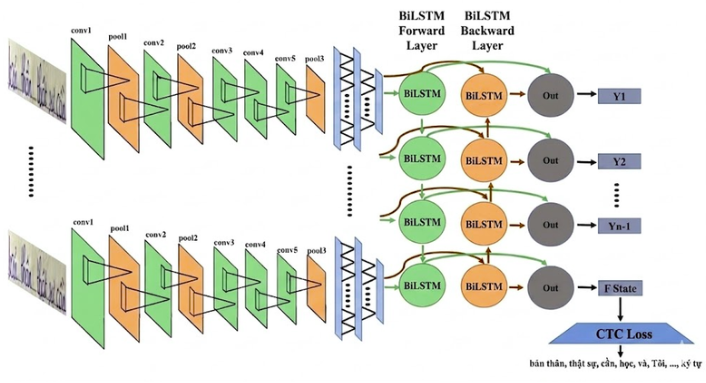
\includegraphics[width=0.9\linewidth]{Figures/Chapter3/Chapter3_8.png}
    \caption{Hình ảnh mạng CRNN}
    \label{fig:handwriting_challenges}
\end{figure}

\subsection*{1. Ảnh đầu vào}
Hệ thống không xử lý trực tiếp toàn bộ ảnh lớn mà sử dụng các ảnh đã được cắt (crop) từ Module 1. Mỗi ảnh đầu vào chỉ chứa một dòng chữ viết tay duy nhất. Cách tiếp cận này giúp đơn giản hóa bài toán, cho phép mô hình tập trung vào việc nhận diện chuỗi ký tự theo thứ tự từ trái sang phải, đồng thời giảm nhiễu từ các vùng không liên quan.

\subsection*{2. Trích xuất đặc trưng}
Ảnh đầu vào được đưa qua các lớp tích chập (CNN) để trích xuất đặc trưng hình ảnh\cite{Reference5,Reference16}. CNN đóng vai trò như một bộ trích xuất đặc trưng, có khả năng phát hiện các thành phần cơ bản như nét dọc, nét ngang, đường cong và cấu trúc hình học của ký tự.

Đầu ra của bước này là một chuỗi đặc trưng (feature sequence), trong đó ảnh được biểu diễn dưới dạng các vector đặc trưng theo từng vị trí từ trái sang phải. Có thể hình dung quá trình này như việc chia ảnh thành nhiều lát cắt dọc, mỗi lát chứa thông tin của một phần chữ viết.

\subsection*{3. Học ngữ cảnh chuỗi}
Do chữ viết tay thường có hiện tượng dính ký tự và khó phân tách, mô hình sử dụng mạng BLSTM (Bidirectional Long Short-Term Memory) để học ngữ cảnh \cite{Reference5,Reference6}.

BLSTM xử lý chuỗi đặc trưng theo hai chiều: từ trái sang phải và từ phải sang trái. Nhờ đó, mô hình có thể tận dụng thông tin ngữ cảnh ở cả hai phía để dự đoán chính xác ký tự, đặc biệt trong các trường hợp ký tự bị mờ hoặc không rõ ràng.

\subsection*{4. Phân loại và dự đoán ký tự}
Sau khi đã học được ngữ cảnh, dữ liệu được đưa qua các lớp Fully Connected để thực hiện phân loại. Lớp cuối cùng sử dụng hàm Softmax để tính toán xác suất của từng ký tự trong bảng chữ cái tiếng Việt tại mỗi vị trí trong chuỗi.

Kết quả đầu ra là một chuỗi các xác suất tương ứng với các ký tự dự đoán.

\subsection*{5. CTC}
Để chuyển đổi chuỗi dự đoán thành văn bản hoàn chỉnh, mô hình sử dụng thuật toán CTC Loss, cho phép ánh xạ chuỗi đầu ra có độ dài thay đổi thành chuỗi ký tự cuối cùng bằng cách loại bỏ các ký tự lặp và ký tự rỗng (blank) \cite{Reference7}.

\subsection{Tiền xử lý ảnh}

Khi scan hoặc chụp ảnh tài liệu, các dòng chữ thường không nằm ngang hoàn hảo mà sẽ bị nghiêng. Nếu đưa ảnh nghiêng trực tiếp vào mạng CRNN, các lát cắt dọc sẽ cắt chéo qua nét chữ, làm giảm độ chính xác nghiêm trọng. Quy trình Deskew (Chỉnh nghiêng) bằng Hough Transform được áp dụng để giải quyết vấn đề này.

\begin{figure}[H]
\centering

\vspace{0.5cm}

\resizebox{0.85\textwidth}{!}{
\begin{tikzpicture}[
    >={Stealth[length=2.5mm, width=1.5mm]},
    base box/.style={
        rectangle, rounded corners=6pt,
        minimum width=4cm, minimum height=1.4cm,
        align=center, font=\sffamily\small\bfseries,
        line width=1pt
    },
    box input/.style={base box, fill=blue!5, draw=blue!60},
    box process/.style={base box, fill=cyan!5, draw=cyan!70},
    box output/.style={base box, fill=green!5, draw=green!60},
    line/.style={->, draw=gray!60!black, line width=1.2pt}
]

% Nodes
\node[box input]   (step1) at (0, 0)      {Ảnh Đầu Vào\\(Bị nghiêng)};
\node[box process] (step2) at (5.5, 0)    {Tiền xử lý\\Binary};
\node[box process] (step3) at (11.0, 0)   {Phát hiện Cạnh\\Canny};

\node[box process] (step4) at (11.0, -2.5) {Chuyển đổi Hough\\(Tìm góc $\theta_{peak}$)};
\node[box process] (step5) at (5.5, -2.5)  {Xoay ảnh\\(Góc $-\theta_{peak}$)};
\node[box output]  (step6) at (0, -2.5)    {Ảnh Đầu Ra\\(Đã Deskew)};

% Arrow
\draw[line] (step1) -- (step2);
\draw[line] (step2) -- (step3);
\draw[line] (step3) -- (step4);
\draw[line] (step4) -- (step5);
\draw[line] (step5) -- (step6);

\end{tikzpicture}
}

\caption{Quá trình xử lý dòng chữ}
\label{fig:data_pipeline}

\end{figure}

% \vspace{0.3cm} % Tạo khoảng trống giữa hình và văn bản

\textbf{Công thức chuyển đổi Hough Transform:}
\begin{equation}
    \rho = x \cos \theta + y \sin \theta
\end{equation}

Trong đó, các đại lượng được định nghĩa cụ thể như sau:
\begin{itemize}
    \item \textbf{$(x, y)$:} Tọa độ của một điểm ảnh (pixel) bất kỳ trong không gian ảnh ban đầu (thường là các điểm thuộc nét chữ đã được trích xuất sau bước phát hiện cạnh Canny).
    \item \textbf{$\rho$ (Rho):} Khoảng cách vuông góc tính từ gốc tọa độ (thường là góc trên cùng bên trái của ảnh) đến đường thẳng đang xét.
    \item \textbf{$\theta$ (Theta):} Góc tạo bởi trục hoành ($x$) và đoạn thẳng vuông góc nối từ gốc tọa độ đến đường thẳng đó. Giá trị $\theta$ này đại diện cho độ nghiêng của dòng chữ.
\end{itemize}


\textbf{Nguyên lý hoạt động trong không gian tham số:}

Thay vì sử dụng phương trình đường thẳng dạng $y = ax + b$ (gặp khó khăn khi đường thẳng đứng có hệ số góc $a$ tiến tới vô cùng), Hough Transform chuyển bài toán sang không gian tham số $(\rho, \theta)$. 

\begin{itemize}
    \item Với mỗi điểm $(x, y)$ trong không gian ảnh, có vô số đường thẳng đi qua nó, tương ứng với một đường cong hình sin trong không gian $(\rho, \theta)$.
    \item Nếu nhiều điểm $(x, y)$ cùng nằm trên một đường thẳng, các đường cong hình sin tương ứng của chúng sẽ giao nhau tại một điểm duy nhất $(\rho_{peak}, \theta_{peak})$.
    \item Điểm giao nhau này chính là "phiếu bầu" cao nhất, giúp thuật toán xác định được góc nghiêng chính xác của dòng chữ để thực hiện phép xoay (Deskew) về trạng thái nằm ngang ($\theta = 0^\circ$).
\end{itemize}

\subsubsection*{1. Ảnh đầu vào}

Hệ thống nhận một hình ảnh dòng chữ viết tay đã được crop, nhưng nó đang bị xô lệch (ví dụ góc nghiêng ban đầu $\theta_{skew} \approx +5.8^\circ$).

\subsubsection*{2. Quy trình deskew}
Quy trình này gồm 4 bước nối tiếp nhau để tìm và sửa lỗi nghiêng:
    \begin{itemize}
        \item \textbf{Tiền xử lý Binary (Binary Conversion):} Ảnh gốc (thường có màu xám hoặc nhiễu) được chuyển hóa thành dạng nhị phân (chỉ gồm 2 màu đen và trắng). Việc này giúp tách bạch hoàn toàn phần nét chữ (foreground) ra khỏi phần giấy nền (background).
        \item \textbf{Phát hiện cạnh Canny (Canny Edge Detection):} Thay vì xử lý toàn bộ các điểm ảnh nét chữ, thuật toán Canny sẽ quét qua ảnh nhị phân và chỉ giữ lại các đường viền (cạnh). Điều này làm giảm đáng kể khối lượng dữ liệu, chỉ giữ lại bộ khung hình học giúp phát hiện đường thẳng.
        \item \textbf{Chuyển đổi Hough (Hough Transform):} Đây là bước cốt lõi để tìm ra góc nghiêng của dòng chữ. Thuật toán xét từng điểm ảnh trên các đường cạnh Canny và ánh xạ chúng sang không gian Hough (dưới dạng các đường cong hình sin). Nơi các đường cong này giao nhau nhiều nhất (điểm $\theta_{peak}$) chính là góc nghiêng thực tế của dòng chữ.
        \item \textbf{Xoay (Rotation):} Khi đã biết chính xác dòng chữ đang bị nghiêng ở góc $\theta_{peak}$ (ví dụ $+5.8^\circ$), hệ thống áp dụng phép xoay hình học để bẻ ngược bức ảnh lại một góc bù trừ ($-\theta_{peak}$).
    \end{itemize}

\subsubsection*{3. Đầu ra}

Kết quả cuối cùng là một bức ảnh chứa dòng chữ đã được điều chỉnh cho nằm ngang hoàn hảo (góc $0^\circ$). Bức ảnh ngay ngắn này giờ đây đã sẵn sàng để được đưa vào mạng CRNN để trích xuất đặc trưng và nhận diện.

\subsection{Quá trình làm dữ liệu}

Quy trình chuẩn bị dữ liệu và huấn luyện mô hình được thực hiện qua các giai đoạn nghiêm ngặt nhằm đảm bảo độ chính xác tối ưu cho hệ thống nhận dạng. Các bước cụ thể được mô tả như sau:

\begin{figure}[H]
\centering

\resizebox{\textwidth}{!}{
\begin{tikzpicture}[
    >={Stealth[length=2.5mm, width=1.5mm]},
    base box/.style={
        rectangle, rounded corners=6pt,
        minimum width=3.6cm, minimum height=1.2cm,
        align=center, font=\sffamily\small\bfseries,
        line width=1pt
    },
    decision box/.style={
        diamond, aspect=2, 
        minimum width=4cm, minimum height=1.5cm,
        align=center, font=\sffamily\small\bfseries,
        line width=1pt,
        fill=orange!5, draw=orange!60
    },
    box input/.style={base box, fill=blue!5, draw=blue!60},
    box process/.style={base box, fill=cyan!5, draw=cyan!70},
    box bad/.style={base box, fill=red!5, draw=red!50},
    box train/.style={base box, fill=teal!5, draw=teal!70},
    edge label/.style={
        font=\sffamily\small\bfseries, text=gray!70!black
    },
    line/.style={->, draw=gray!60!black, line width=1.2pt},
    noline/.style={draw=gray!60!black, line width=1.2pt}
]

% ===== NODES =====
\node[box input]     (raw)      at (0, 0)      {Raw Text Line Images};
\node[box process]   (manual)   at (4.8, 0)    {Manual Annotation};
\node[box process]   (filter)   at (9.6, 0)    {Quality Filtering};

\node[decision box]  (valid)    at (14.8, 0)   {Valid Text\\Line?};

\node[box bad]       (remove)   at (20, 2.5)   {Remove Low-Quality\\Samples};
\node[box train]     (traindata)at (20, -2.5)  {Training Dataset};

\node[box train]     (traincrnn)at (25, -2.5)  {Train CRNN Model};

% ===== MAIN FLOW =====
\draw[line] (raw) -- (manual);
\draw[line] (manual) -- (filter);
\draw[line] (filter) -- (valid);

% ===== FORK POINT (RA GIỮA KHÔNG MŨI TÊN) =====
\coordinate (fork) at ($(valid.east) + (0.15,0)$);

\draw[noline] (valid.east) -- (fork);

% % (optional) chấm fork cho đẹp
% \fill (fork) circle (2pt);

% ===== NHÁNH NO =====
\draw[line]
(fork) -- ++(0,1.6) |- (remove.west);

\node[edge label] at ($(fork)+(0.6,1.3)$) {No};

% ===== NHÁNH YES =====
\draw[line]
(fork) -- ++(0,-1.6) |- (traindata.west);

\node[edge label] at ($(fork)+(0.6,-1.3)$) {Yes};

% ===== TRAIN FLOW =====
\draw[line] (traindata) -- (traincrnn);

\end{tikzpicture}
}

\caption{Quá trình xử lý dữ liệu}
\label{fig:data_pipeline}

\end{figure}

\begin{itemize}
    \item \textbf{Raw Text Line Images (Dữ liệu thô):} Tập hợp các hình ảnh dòng văn bản được cắt trích ra sau quá trình phát hiện dòng chữ của module 1.
    
    \item \textbf{Manual Annotation (Gán nhãn thủ công):} Sử dụng một tool label tự tạo để gán nhãn thủ công chuyển đổi thông tin từ dạng hình ảnh sang định dạng văn bản kỹ thuật số. Bước này tạo ra tập dữ liệu đối sánh chuẩn (\textit{ground-truth}) phục vụ cho việc giám sát quá trình học của máy.
    
    \item \textbf{Quality Filtering (Lọc nhiễu và Kiểm soát chất lượng):} Sau khi gán nhãn, dữ liệu được đưa qua bộ lọc để đánh giá tính hợp lệ (\textit{Valid Text Line?}). Quá trình này rẽ nhánh dựa trên chất lượng mẫu:
    \begin{itemize}
        \item \textit{Trường hợp không đạt (No):} Các mẫu có hình ảnh mờ nhòe hoặc nhãn sai lệch sẽ bị loại bỏ thông qua bước \textbf{Remove Low-Quality Samples}.
        \item \textit{Trường hợp đạt chuẩn (Yes):} Các dữ liệu tinh sạch sẽ được đưa vào \textbf{Training Dataset}.
    \end{itemize}
    
    \item \textbf{Train CRNN Model (Huấn luyện mô hình):} Sử dụng tập dữ liệu đã qua sàng lọc để huấn luyện mạng nơ-ron tích chập tuần tự (\textit{Convolutional Recurrent Neural Network - CRNN}), giúp mô hình học cách ánh xạ từ đặc trưng hình ảnh sang chuỗi ký tự văn bản \cite{Reference5}.
\end{itemize}
\subsection{Dataset}

Để huấn luyện mô hình CRNN (Convolutional Recurrent Neural Network) cho bài toán nhận dạng chữ, tập dữ liệu đầu vào bao gồm các hình ảnh chứa các dòng văn bản đã được cắt ra (crop) từ giai đoạn phát hiện (detection) trước đó. Các hình ảnh này được thu thập với sự biến dạng về bối cảnh, góc chụp và điều kiện ánh sáng để tăng cường khả năng tổng quát hóa của mô hình. Toàn bộ dữ liệu được phân chia theo tỉ lệ: 80\% cho tập huấn luyện (Train), 15\% cho tập kiểm tra (Validation) và 5\% cho tập đánh giá (Test).
\begin{table}[h]
    \centering
    \begin{tabular}{lcc}
        \toprule
        \textbf{Tập dữ liệu} & \textbf{Số ảnh} & \textbf{Số nhãn} \\
        \midrule
        Train      & 1534 & 1534 \\
        Validation & 285  & 285  \\
        Test       & 94  & 94  \\
        \bottomrule
    \end{tabular}
    \caption{Thống kê tập dữ liệu hình ảnh dòng chữ.}
    \label{tab:detection_dataset}
\end{table}

\subsection{Hàm mất mát}

Trong các bài toán nhận dạng chuỗi như nhận dạng chữ viết (OCR), sự gióng hàng (alignment) giữa chuỗi đặc trưng đầu vào và chuỗi ký tự đầu ra thường không được biết trước do sự chênh lệch về độ dài. Để giải quyết triệt để vấn đề này, mô hình sử dụng hàm mất mát \textbf{CTC (Connectionist Temporal Classification)} \cite{Reference7}.

\begin{itemize}
    \item \textbf{Xác suất chuỗi trong CTC:}
    
    Xác suất để mô hình dự đoán đúng chuỗi mục tiêu $y$ khi cho trước đầu vào $x$ được định nghĩa là tổng xác suất của tất cả các đường dẫn (paths) hợp lệ có thể sinh ra $y$:
    $$P(y|x) = \sum_{\pi \in B^{-1}(y)} P(\pi|x)$$
    
    Trong đó, do giả định các dự đoán tại mỗi thời điểm là độc lập, xác suất của một đường dẫn cụ thể $\pi$ được tính bằng tích các xác suất dự đoán tại từng bước thời gian $t$:
    $$P(\pi|x) = \prod_{t=1}^{T} p_{\pi_t}^{(t)}$$

    \textbf{Giải thích các đại lượng:}
    \begin{itemize}
        \item $x$: Chuỗi đặc trưng đầu vào (được trích xuất từ các lớp mạng nơ-ron trước đó).
        \item $y$: Chuỗi nhãn thực tế (\textit{ground-truth}) cần dự đoán.
        \item $\pi$: Một đường dẫn dự đoán thô ở cấp độ từng khung hình (\textit{frame}). Đường dẫn này có độ dài bằng $T$, bao gồm cả các ký tự lặp lại và ký hiệu rỗng (\textit{blank}).
        \item $B$: Hàm ánh xạ (thu gọn) làm nhiệm vụ loại bỏ các ký tự lặp lại liền kề và các ký hiệu rỗng từ đường dẫn thô $\pi$ để tạo ra chuỗi đầu ra cuối cùng.
        \item $B^{-1}(y)$: Tập hợp tất cả các đường dẫn $\pi$ hợp lệ mà sau khi đi qua hàm ánh xạ $B$ sẽ tạo thành chuỗi mục tiêu $y$.
        \item $T$: Tổng số bước thời gian (\textit{time steps}) của đặc trưng đầu vào.
        \item $p_{\pi_t}^{(t)}$: Xác suất mà mạng nơ-ron dự đoán ra ký tự $\pi_t$ tại thời điểm $t$.
    \end{itemize}

    \item \textbf{Hàm mất mát CTC Loss:}
    
    Mục tiêu cốt lõi của quá trình huấn luyện là cực đại hóa xác suất dự đoán đúng $P(y|x)$. Tương tự như hàm Cross-Entropy, để thuận tiện cho các thuật toán tối ưu hóa (như Gradient Descent), CTC Loss sử dụng hàm logarit âm (\textit{Negative Log-Likelihood}):
    $$\mathcal{L}_{CTC} = -\log P(y|x)$$
    
    Việc cực tiểu hóa giá trị lỗi $\mathcal{L}_{CTC}$ tương đương với việc cực đại hóa xác suất $P(y|x)$. Thông qua quá trình lan truyền ngược (\textit{backpropagation}), mạng nơ-ron sẽ tự động điều chỉnh các trọng số để mô hình đưa ra dự đoán tiệm cận nhất với nhãn thực tế.
\end{itemize}

